% The bond (zero-site) effective Hamiltonian, applied to the centre on a bond:
% H_eff C.
%
% Factor the centre off a site, AC = AL C, let AL join the left environment,
% and the centre is C, on the bond. C carries no physical index, so nothing of
% the Hamiltonian sits here: the MPO's bond runs straight from L to R, which is
% the `-' slot -- a layer whose index passes through. One-site TDVP evolves C
% backwards in time with this, and VUMPS solves for its fixed point.
%
% The slot is the same width as a site's. The centre on a bond is a different
% shape (the small diamond) rather than a different slot.
\documentclass[border=4pt]{standalone}
\usepackage{amsmath,amssymb}
\usepackage{tikz-tensors}
\input{notation}
\begin{document}
\begin{tikzpicture}
  \tnstack[left=$L$, right=$R$]{K}{1}{ket, op, bra}
  \tnlayer{K}{ket}{centrebond/$C$}
  \tnlayer{K}{op}{-}
  \tnconnect{K}
  \tnput[below]{K-bra-left}{$a$}
  \tnput[below]{K-bra-right}{$b$}
\end{tikzpicture}
\end{document}
